
\documentclass[11pt]{article}
\usepackage{graphicx}
\usepackage{listings}
\usepackage{multirow}
\usepackage{color}
\usepackage[english]{babel}
\usepackage{mylingmacros}

\newcommand\add[1]{{\textcolor{blue}{ADD: #1}}}
\newcommand\mod[1]{{\textcolor{green}{MODIFIED: #1}}}
\newcommand\remove[1]{{\textcolor{red}{REMOVE: #1}}}
\newcommand\expand[1]{{\textcolor{blue}{EXPAND: #1}}}
\newcommand\rewrite[1]{{\textcolor{green}{REWRITE: #1}}}

% Titre complet


\title{Report}

\author{Anna Liednikova}


\begin{document}

\maketitle

\tableofcontents

\clearpage

\section{Introduction}

 
This project was set within the framework of a collaboration with the
ALIAE startup where the aim is to develop a chatbot to collect
information from clinical patients. The main idea is to replace
strictly defined surveys by a more natural conversation in order to
let users express themselves freely so that more information could be
collected.


\add{The chatbot consists of three main modules: NLU (Natural
  Language Understanding: interpreting the user input), Dialog
  Managment (Deciding on how to respond to the user input) and NLG
  (Generating the system response).}

\add{In this project, we focus on the NLU step which consists in}
analysing the user utterance (does the user speaks about pain,
physical activity etc. ?) and detecting at least one most probable
intent of user message so that the chatbot can choose the right
strategy for fulfilling information.

\add{ADD an example showing a user input and the expected representation ie intent + entity}


A small manually annotated dataset (roughly 100 sentences for each
category) was available.

\add{say that this dataset is not enough for learning a good NLU models. Hence your work focuses on exploring automatic ways of extending the training data and 
  learning NLU models from these extended data.}

\add{Explain report structure: which section focuses on what?}


\remove{We have tried models for sentence representation by word and the whole context in order to use semi-supervised learning by gradually increasing train data by labelling external sources.}

\section{Literature review}

\cite{N18-2058} \mod{present an approach for automatically generating additional training data for event extraction systems}. First, they trained a baseline classifier on available data. Then, they cluster external data to obtain cluster of paraphrases using the NewsSpike method introduced by \cite{zhang2015}. They then label the clusters using the baseline model trained on the initial dataset of labelled data. Combining the new labelled data and the original one, they then retrained the event extractor.

\section{Methodology}

\add{We follow \cite{N18-2058} methodology. Instead of using \cite{zhang2015}'s methods for identifying clusters of related sentences however, we explore different ways of representing sentences using deep learning approaches. We then apply clustering to the resulting sentence representations. Finally, we investigate the impact of the extended labeled data on classification. }

%% irst
%% group together paraphrases of event mentions.

%% then use the simple examples in each cluster to as-
%% sign a label to the entire cluster

%% com-
%% bine the new examples with the original training
%% set and retrain


\subsection{Building Sentence Representations}

We create sentence representations in two steps using machine and deep learning techniques. First, we map words to continuous representations. Second, we combine these word representations into sentence representations. 

\subsubsection{Word Representations}

We explore two ways of building word representations: Word2vec and LDA.

\add{You need to explain what LDA and Word2Vec are and how they represent word/sentences}


\remove{The most popular word-basis techniques to represent sentences are LDA (Latent Dirichlet Allocation) and Word2Vector model. We used their implementation from gensim library in order to build models based on the initial labelled dataset.
}

\subsubsection{Sentence Representations}

\mod{We construct sentence representations out of the word representations described in the previous section using two types of neural networks:  PositionwiseFeedForward \cite{vaswani2017attention} and BiLSTM \add{bibref}}.

\add{Here you need to explain the theory behind it. Explain how LSTM and the PositionwiseFeedForward  build a sentence representation out of word embeddings.}

\paragraph{Bi-LSTM Representations.}


\paragraph{Tranformer Representations.}

<<<<<<< HEAD
=======
The most popular word-basis techniques to represent sentences are LDA (Latent Dirichlet Allocation) and Word2Vector models. We used their implementation from gensim library in order to build models based on the initial labelled dataset.

Preprocessed tokenized sentences were used to create dictionary and were passed to W2V model as it is and in form of Bag-Of-Word to LDA model.

For selecting the best model we changed space dimension (topics for LDA and features for W2W). Preferred number of features for W2V model is 200. It's the start point for our model.

The good point of using this models is that they can be used for both word and sentence representation since one word can be treated as a small sentence.
>>>>>>> 1fd91297f0d748d6268bc796f027ba6b4c129a5a



\subsection{Clustering Sentences}

\mod{Using the sentence representations described in the previous
  section, we apply clustering to group together sentences that are
  similar. We compare three clustering algorithms:}

\add{Briefly explain the key feature of each clustering algorithm}


\begin{itemize}
\item K-Means (KM)
\item AgglomerativeClustering(‘ward’) (AG)
\item GaussianMixture (GM)
\end{itemize}

<<<<<<< HEAD
We set the number of clusters to the number of intents (20)
which allows using not only purity and Silhouette coefficients to
evaluate the clusters but also homogeneity and completeness to get the
idea how resulting groups correlate with initial intents. Also, for
each model, we plot a confusion matrix with a background gradient
to visualize how well clusters separate different intents.

\subsection{Classifying Sentences}

Train on labelled data
=======
The number of clusters was set to the number of intents (20) that allows using not only purity and Silhouette coefficients to evaluate them but also homogeneity and completeness to get the idea how resulting groups correlate with initial intents. Also, for each model, we plotted a confusion matrix with a background gradient to visualize how well clusters separate different intents.
>>>>>>> 1fd91297f0d748d6268bc796f027ba6b4c129a5a

Test on unlabelled data

\section{Datasets}

\subsection{Labelled Data}

The initial dataset is created manually covering 20 main possible users intents. Each sentence represents one intent. For, example,

\enumsentence{
\textbf{Text:} After sleep, for 2-3 hours, I am better and then start feeling tired again\\
\textbf{Intent:} sleep
}

The distribution of labels is shown in Figure~\ref{figure:name}. There
are in average, 3.4 words per sentence (min: 0, max: 12, std:
2.16367).  The total number of sentences is 3305 and the vocabulary
consists of 1882 content words (after removing stopwords).

 \begin{figure}[h]
 	\centering
 	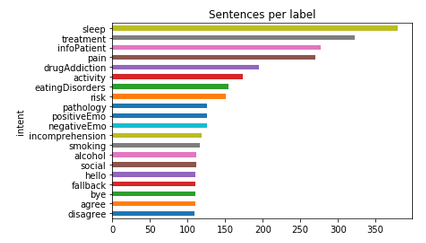
\includegraphics[scale=0.5]{report1.png}
	\caption{Label distribution in dataset}
 \label{figure:name}
 \end{figure}




 \begin{figure}[h]
 	\centering
 	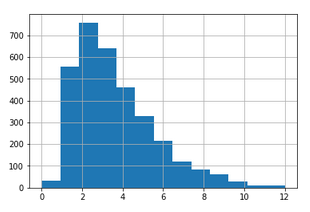
\includegraphics[scale=0.4]{report4.png}
	\caption{Sentence dist}
 \label{words_freq}
 \end{figure}



\subsection{Forum data}

To create additional training data, we extracted textual data from
HealthBoards \add{URL}, a medical forum web portal that allows
patients to discuss their ailments.

We scraped 272,553 unique posts contained in each category.  The post
were then segmented into sentences, tokenized and lemmatized using NLP
libraries. Stop words were removed.

We compared two libraries, NLTK and SpaCy.

For example, in word tokenization they give different results that can influence not only simple statistics but meaning too. Some example of different tokenization can be seen in table \ref{token_dif}. Though concating words to ones like 'flulike' or '35mg' or 'longterm' sometimes gives more robust and concrete meaning in case of big dataset, in our case it seems better to stay with spacy way of tokenization in order to have smaller and more simple vocabualary.

For stopwords removing there were three options: nltk, spacy and the longest one. The last option was rejected due to containing words like 'want', 'stop', 'successfully' etc. that can be useful for detecting basic intents like positive or negative emotion, social. Finally nltk one was selecting because of containing shorts like 'm' from 'am', 've' from 'have'. Final dictionary contained 1882 words. Also all numbers were changed to num. Chart (\ref{words_freq}) looks fine.

 \begin{figure}[h]
 	\centering
 	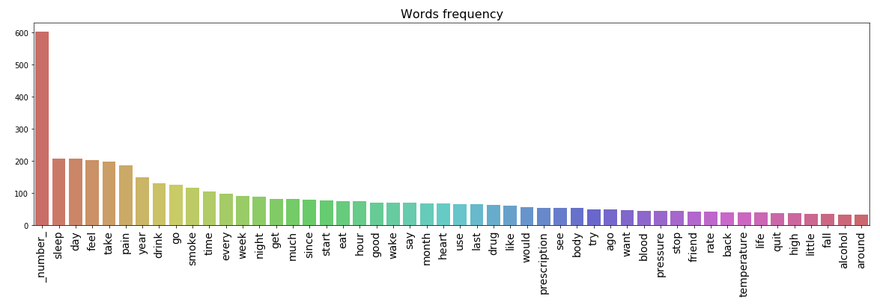
\includegraphics[scale=0.4]{report2.png}
	\caption{Words frequency}
 \label{words_freq}
 \end{figure}

Length < 30.


Next problem is empty sentences. But they don't change the dataset much.

intent
fallback           12
disagree           11
hello               4
agree               3
incomprehension     2
positiveEmo         1

array(['what?', 'same that again', 'I am up', 'same', 'can you',
       'do that', 'do this', 'Will do', 'no', 'no i will not',
       "No i don't", 'no', 'no i will not', "No i don't", "What's up?",
       "What's up?", 'he', 'a', 'd', 'i', 'm', 'o', 's', 't', 'y',
       'I will', 'Will do', 'No', 'no', 'No it is not', "No I don't",
       'No', "I'm here"], dtype=object)

\begin{center}
\begin{table}
\begin{tabular}{ |p{7cm}|p{7cm}| }
\hline
NLTK & SpaCy \\ \hline
['i', 'wouldnt', 'go', 'to', 'sleep', 'until', 'like', '5', '6', 'or', '8am'] & 
['i', 'would', 'nt', 'go', 'to', 'sleep', 'until', 'like', '5', '6', 'or', '8', 'am'] \\ \hline
['that', 'is', 'totally', 'wrongheaded'] & ['that', 'is', 'totally', 'wrong', 'headed'] \\ \hline
['i', 'am', 'in', 'the', 'process', 'of', 'tapering', 'from', 'suboxone', 'longterm', 'use'] & 
['i', 'am', 'in', 'the', 'process', 'of', 'tapering', 'from', 'suboxone', 'long', 'term', 'use'] \\ \hline
['i', 'had', 'an', 'onandoff', 'opiateopioid', 'habit', 'from', 'about', '2010'] & 
['i', 'had', 'an', 'on', 'and', 'off', 'opiate', 'opioid', 'habit', 'from', 'about', '2010'] \\ 
\hline
['i', 'have', 'flulike', 'pathologysymptom'] & ['i', 'have', 'flu', 'like', 'pathologysymptom'] \\ \hline
['i', 'have', 'exerciseinduced', 'insomnia'] & ['i', 'have', 'exercise', 'induced', 'insomnia'] \\ \hline
['i', 'm', 'supposed', 'to', 'take', '6', '35mg', 'tablets', 'a', 'day', 'but', 'i', 'have', 'taken', '20', 'today'] & 
['i', 'm', 'supposed', 'to', 'take', '6', '35', 'mg', 'tablets', 'a', 'day', 'but', 'i', 'have', 'taken', '20', 'today'] \\ 
\hline
\end{tabular}	
\caption{\label{token_dif}Tokenization comparison}
\end{table}
\end{center}


Finally, the corpus consists of N  sentences. Table \ref{tab:datastats} and Figure~\ref{visina8} show the dataset statistics.


{'min': 0, 'max': 2027, 'mean': 10.932588521491454, 'std': 8.964716092053479}
{'min': 3.2580388329566468, 'max': 35.23600634007455, 'mean': 11.224462266261876, 'std': 6.963225985041148}

\begin{table}
\begin{tabular}{ |l|rrr| }
  \hline
   & \# Sentence & Avg Stce Size (min/max) & Vocab. Size\\\hline
  Unlabelled Data & 3305 & 3.4 (0/12) & 1882 \\
  Labelled Data & & 10.93 (0/2027) & \\\hline
\end{tabular}
\caption{Labelled and Unlabelled Data}
\label{tab:datastats}
\end{table}
 \begin{figure}[h]
 	\centering
 	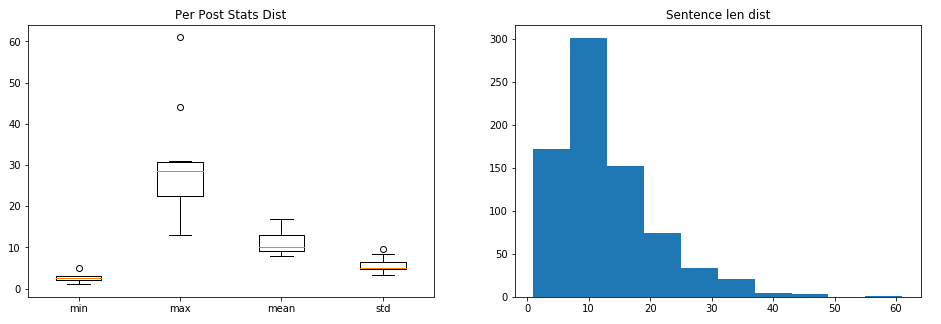
\includegraphics[scale=0.5]{report3.png}
	\caption{Text stat}\label{visina8}
 \end{figure}

Data should be divided in subsets by increasing sentence length because of the difference in mean values for both datasets.



\section{Experiment}

\subsection{Clustering}
\subsubsection{Evaluation metrics}
\subsubsection{W2V model}

Comparison table

\begin{tabular}{ |p{2cm}|p{1cm}|c|c|c|c|p{1cm}| }
\hline
WE & Cluster & purity & Silhouette & homogeneity & complete & Clf CV score \\ \hline
\multirow{3}{*}{Defenders} & KM & & & & &\\
 & AC & & & & &\\
 & GM & & & & &\\ \hline
\multirow{3}{*}{M} & KM & & & & &\\
 & AC & & & & &\\
 & GM & & & & &\\ \hline
Forward & FW & & & & &\\ \hline
\multirow{3}{*}{S} & KM & & & & &\\
 & AC & & & & &\\
 & GM & & & & &\\
\hline
\end{tabular}


\subsubsection{LDA model}


\subsubsection{GloVe pretrained}

\subsubsection{Google News W2V pretrained}

\subsubsection{CNN by word}

From simple encoder, w2v, lda, w2v + lda

\subsubsection{BiLSTM by word}

From simple encoder, w2v, lda, w2v + lda

\subsubsection{Overall comparison}

\subsection{Classifier}
\subsubsection{Evaluation metrics}
\subsubsection{Results for each model}


\section{Conclusion}


\section{References}
\bibliographystyle{alpha}
\bibliography{biblio}


\end{document}
